% Options for packages loaded elsewhere
\PassOptionsToPackage{unicode}{hyperref}
\PassOptionsToPackage{hyphens}{url}
%
\documentclass[
]{book}
\usepackage{amsmath,amssymb}
\usepackage{iftex}
\ifPDFTeX
  \usepackage[T1]{fontenc}
  \usepackage[utf8]{inputenc}
  \usepackage{textcomp} % provide euro and other symbols
\else % if luatex or xetex
  \usepackage{unicode-math} % this also loads fontspec
  \defaultfontfeatures{Scale=MatchLowercase}
  \defaultfontfeatures[\rmfamily]{Ligatures=TeX,Scale=1}
\fi
\usepackage{lmodern}
\ifPDFTeX\else
  % xetex/luatex font selection
\fi
% Use upquote if available, for straight quotes in verbatim environments
\IfFileExists{upquote.sty}{\usepackage{upquote}}{}
\IfFileExists{microtype.sty}{% use microtype if available
  \usepackage[]{microtype}
  \UseMicrotypeSet[protrusion]{basicmath} % disable protrusion for tt fonts
}{}
\makeatletter
\@ifundefined{KOMAClassName}{% if non-KOMA class
  \IfFileExists{parskip.sty}{%
    \usepackage{parskip}
  }{% else
    \setlength{\parindent}{0pt}
    \setlength{\parskip}{6pt plus 2pt minus 1pt}}
}{% if KOMA class
  \KOMAoptions{parskip=half}}
\makeatother
\usepackage{xcolor}
\usepackage{color}
\usepackage{fancyvrb}
\newcommand{\VerbBar}{|}
\newcommand{\VERB}{\Verb[commandchars=\\\{\}]}
\DefineVerbatimEnvironment{Highlighting}{Verbatim}{commandchars=\\\{\}}
% Add ',fontsize=\small' for more characters per line
\usepackage{framed}
\definecolor{shadecolor}{RGB}{248,248,248}
\newenvironment{Shaded}{\begin{snugshade}}{\end{snugshade}}
\newcommand{\AlertTok}[1]{\textcolor[rgb]{0.94,0.16,0.16}{#1}}
\newcommand{\AnnotationTok}[1]{\textcolor[rgb]{0.56,0.35,0.01}{\textbf{\textit{#1}}}}
\newcommand{\AttributeTok}[1]{\textcolor[rgb]{0.13,0.29,0.53}{#1}}
\newcommand{\BaseNTok}[1]{\textcolor[rgb]{0.00,0.00,0.81}{#1}}
\newcommand{\BuiltInTok}[1]{#1}
\newcommand{\CharTok}[1]{\textcolor[rgb]{0.31,0.60,0.02}{#1}}
\newcommand{\CommentTok}[1]{\textcolor[rgb]{0.56,0.35,0.01}{\textit{#1}}}
\newcommand{\CommentVarTok}[1]{\textcolor[rgb]{0.56,0.35,0.01}{\textbf{\textit{#1}}}}
\newcommand{\ConstantTok}[1]{\textcolor[rgb]{0.56,0.35,0.01}{#1}}
\newcommand{\ControlFlowTok}[1]{\textcolor[rgb]{0.13,0.29,0.53}{\textbf{#1}}}
\newcommand{\DataTypeTok}[1]{\textcolor[rgb]{0.13,0.29,0.53}{#1}}
\newcommand{\DecValTok}[1]{\textcolor[rgb]{0.00,0.00,0.81}{#1}}
\newcommand{\DocumentationTok}[1]{\textcolor[rgb]{0.56,0.35,0.01}{\textbf{\textit{#1}}}}
\newcommand{\ErrorTok}[1]{\textcolor[rgb]{0.64,0.00,0.00}{\textbf{#1}}}
\newcommand{\ExtensionTok}[1]{#1}
\newcommand{\FloatTok}[1]{\textcolor[rgb]{0.00,0.00,0.81}{#1}}
\newcommand{\FunctionTok}[1]{\textcolor[rgb]{0.13,0.29,0.53}{\textbf{#1}}}
\newcommand{\ImportTok}[1]{#1}
\newcommand{\InformationTok}[1]{\textcolor[rgb]{0.56,0.35,0.01}{\textbf{\textit{#1}}}}
\newcommand{\KeywordTok}[1]{\textcolor[rgb]{0.13,0.29,0.53}{\textbf{#1}}}
\newcommand{\NormalTok}[1]{#1}
\newcommand{\OperatorTok}[1]{\textcolor[rgb]{0.81,0.36,0.00}{\textbf{#1}}}
\newcommand{\OtherTok}[1]{\textcolor[rgb]{0.56,0.35,0.01}{#1}}
\newcommand{\PreprocessorTok}[1]{\textcolor[rgb]{0.56,0.35,0.01}{\textit{#1}}}
\newcommand{\RegionMarkerTok}[1]{#1}
\newcommand{\SpecialCharTok}[1]{\textcolor[rgb]{0.81,0.36,0.00}{\textbf{#1}}}
\newcommand{\SpecialStringTok}[1]{\textcolor[rgb]{0.31,0.60,0.02}{#1}}
\newcommand{\StringTok}[1]{\textcolor[rgb]{0.31,0.60,0.02}{#1}}
\newcommand{\VariableTok}[1]{\textcolor[rgb]{0.00,0.00,0.00}{#1}}
\newcommand{\VerbatimStringTok}[1]{\textcolor[rgb]{0.31,0.60,0.02}{#1}}
\newcommand{\WarningTok}[1]{\textcolor[rgb]{0.56,0.35,0.01}{\textbf{\textit{#1}}}}
\usepackage{longtable,booktabs,array}
\usepackage{calc} % for calculating minipage widths
% Correct order of tables after \paragraph or \subparagraph
\usepackage{etoolbox}
\makeatletter
\patchcmd\longtable{\par}{\if@noskipsec\mbox{}\fi\par}{}{}
\makeatother
% Allow footnotes in longtable head/foot
\IfFileExists{footnotehyper.sty}{\usepackage{footnotehyper}}{\usepackage{footnote}}
\makesavenoteenv{longtable}
\usepackage{graphicx}
\makeatletter
\def\maxwidth{\ifdim\Gin@nat@width>\linewidth\linewidth\else\Gin@nat@width\fi}
\def\maxheight{\ifdim\Gin@nat@height>\textheight\textheight\else\Gin@nat@height\fi}
\makeatother
% Scale images if necessary, so that they will not overflow the page
% margins by default, and it is still possible to overwrite the defaults
% using explicit options in \includegraphics[width, height, ...]{}
\setkeys{Gin}{width=\maxwidth,height=\maxheight,keepaspectratio}
% Set default figure placement to htbp
\makeatletter
\def\fps@figure{htbp}
\makeatother
\setlength{\emergencystretch}{3em} % prevent overfull lines
\providecommand{\tightlist}{%
  \setlength{\itemsep}{0pt}\setlength{\parskip}{0pt}}
\setcounter{secnumdepth}{5}
\usepackage{booktabs}
\ifLuaTeX
  \usepackage{selnolig}  % disable illegal ligatures
\fi
\usepackage[]{natbib}
\bibliographystyle{plainnat}
\usepackage{bookmark}
\IfFileExists{xurl.sty}{\usepackage{xurl}}{} % add URL line breaks if available
\urlstyle{same}
\hypersetup{
  pdftitle={BB511 Manual Ion Transport Lab Exercise},
  pdfauthor={Iris Adam},
  hidelinks,
  pdfcreator={LaTeX via pandoc}}

\title{BB511 Manual Ion Transport Lab Exercise}
\author{Iris Adam}
\date{April 2025 v2}

\begin{document}
\maketitle

{
\setcounter{tocdepth}{1}
\tableofcontents
}
\chapter{About}\label{about}

This manual contains the background information for the exercise (Chapter 2) as well as the instructions for each experiment and the data analysis going with it. I am planning to add a markdown template to write your report, but that hasn't happened yet :)

\section{Usage}\label{usage}

This book will take you through the entire exercise step by step and also contain example data so you can analyze and the results after the course.
All code to work with the data is written in code blocks like this:

\begin{Shaded}
\begin{Highlighting}[]
\FunctionTok{print}\NormalTok{(}\StringTok{"BB511 is awesome!"}\NormalTok{)}
\end{Highlighting}
\end{Shaded}

You can directly copy the code from these blocks using the copy button in the upper right corner of the block.

\chapter{Background information}\label{background-information}

Please refer to the Ion transport compendium.

\section{A bit of history}\label{a-bit-of-history}

\section{About Ussing}\label{about-ussing}

\section{The frogs problem}\label{the-frogs-problem}

\chapter{Setting up your equipment}\label{setting-up-your-equipment}

Switch on the equipment and wait 5 minutes. This is necessary for all recording hardware as resistances and capacitors on the circuit boards change with temperature and make the measurements drift while the hardware is heating up.

\section{Building and powering up your setup}\label{building-and-powering-up-your-setup}

\begin{enumerate}
\def\labelenumi{\arabic{enumi}.}
\tightlist
\item
  Assemble your chamber by:
\end{enumerate}

\begin{itemize}
\item
  inserting the slider in between the two chamber halves
\item
  inserting the chamber in the chamber holder
\item
  tightening the screw on the side
\end{itemize}

\begin{enumerate}
\def\labelenumi{\arabic{enumi}.}
\setcounter{enumi}{1}
\tightlist
\item
  Connect \textbf{Voltage} (\textbf{V}, black cables) and \textbf{Current} (\textbf{I}, red and white cables) electrodes.
\end{enumerate}

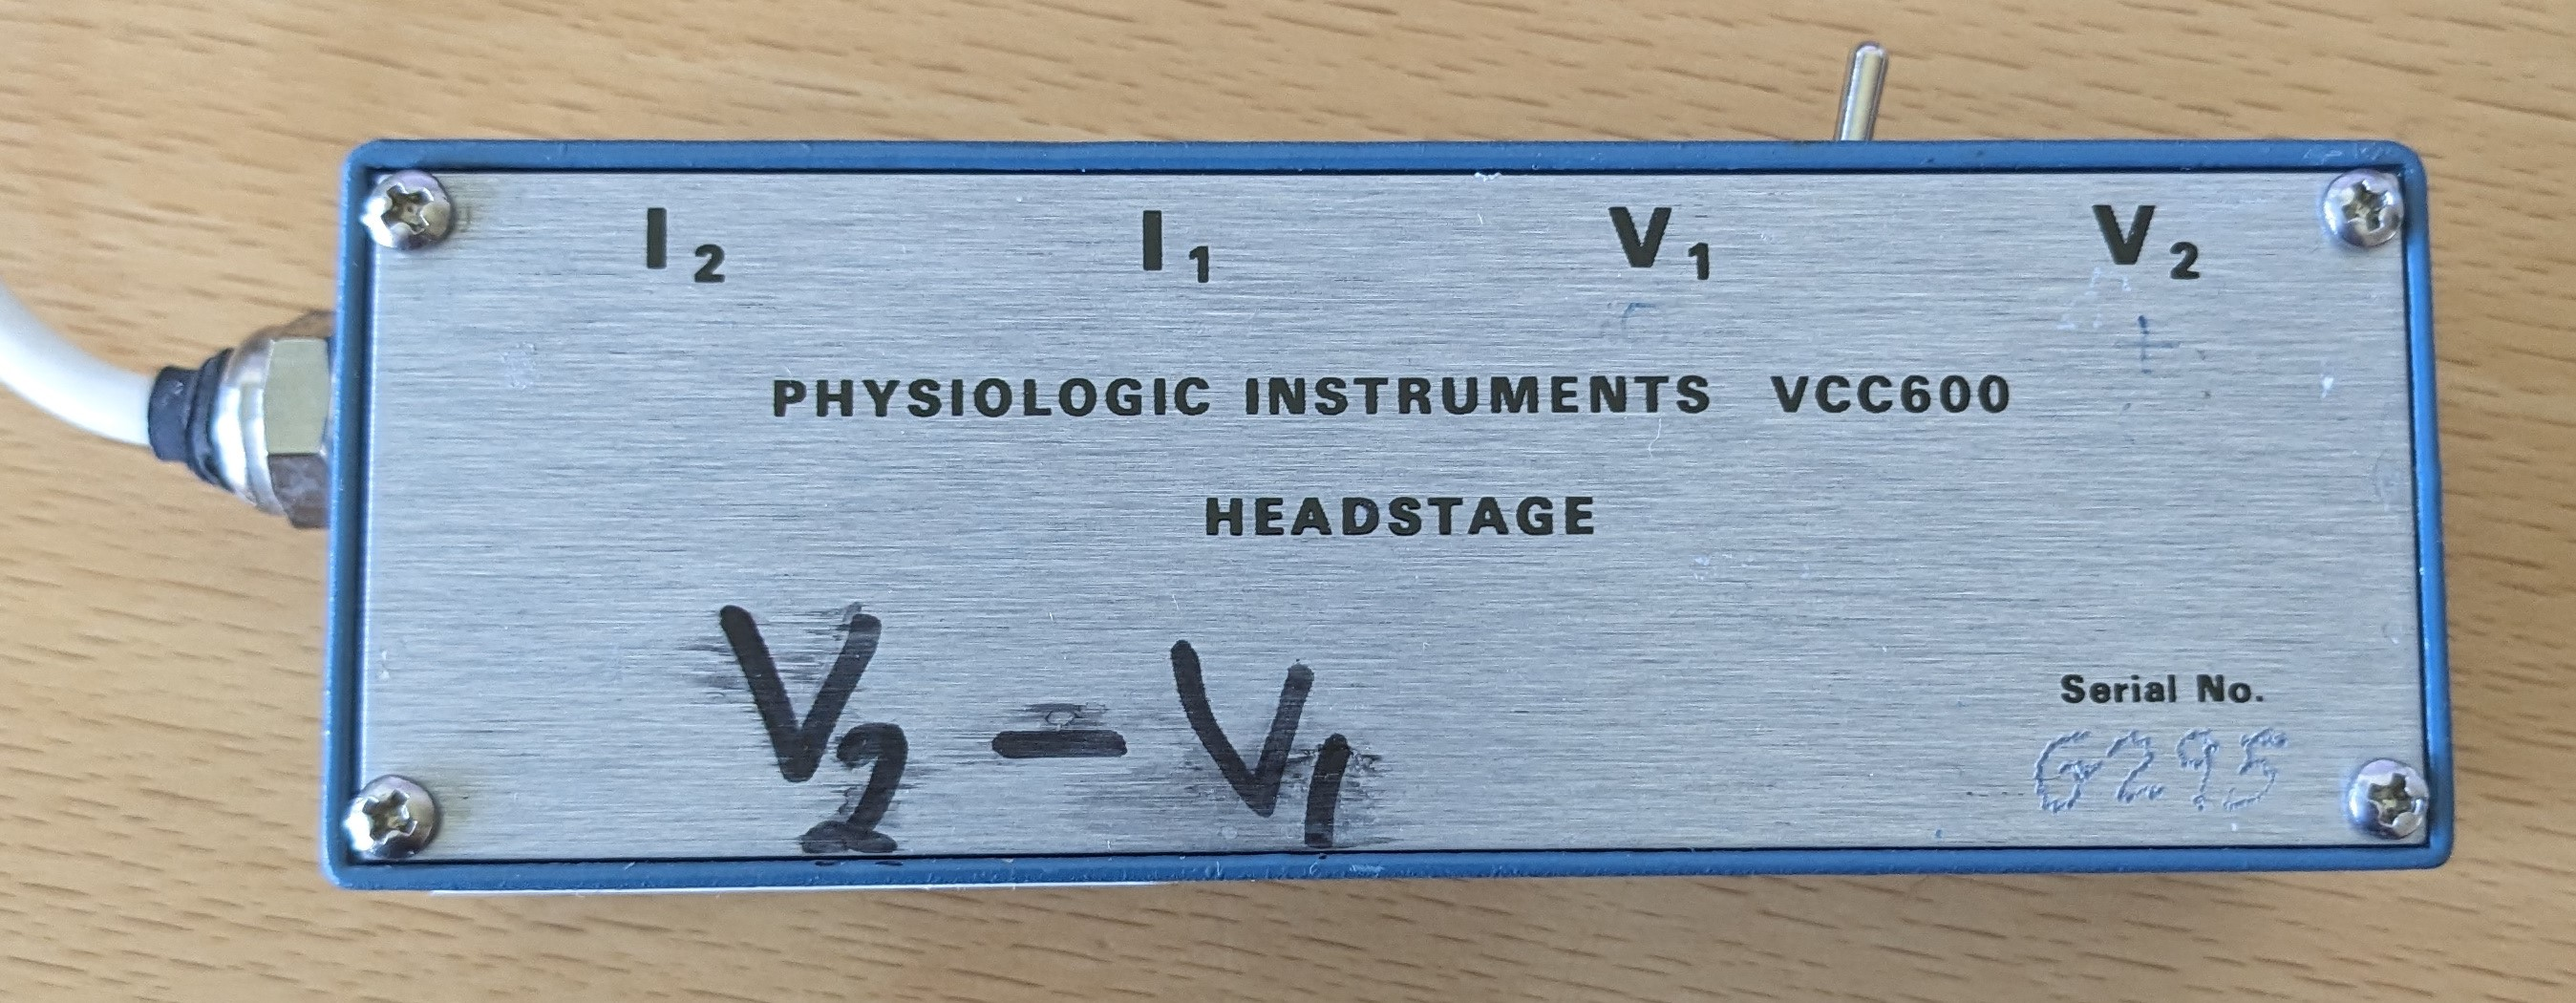
\includegraphics[width=37.46in]{images/headstage}

\begin{enumerate}
\def\labelenumi{\arabic{enumi}.}
\setcounter{enumi}{2}
\tightlist
\item
  Connect electrodes to headstage.
\end{enumerate}

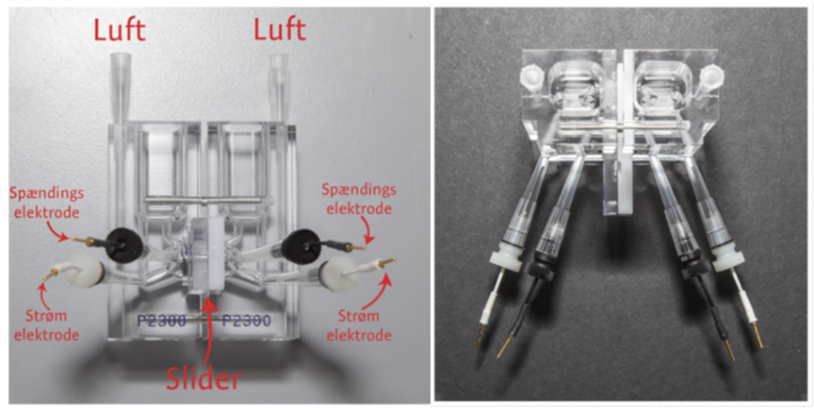
\includegraphics[width=11.31in]{images/Electrode placements}

\begin{enumerate}
\def\labelenumi{\arabic{enumi}.}
\setcounter{enumi}{3}
\item
  Make sure V1 and I1 and V2 and I2 are on the \emph{same side} of the chamber.
\item
  Fill chamber with Ringer's solution, insert tubing that feeds air and start the pump.
\item
  Check that all instrument settings are in the rest setting like on the image below:
\end{enumerate}

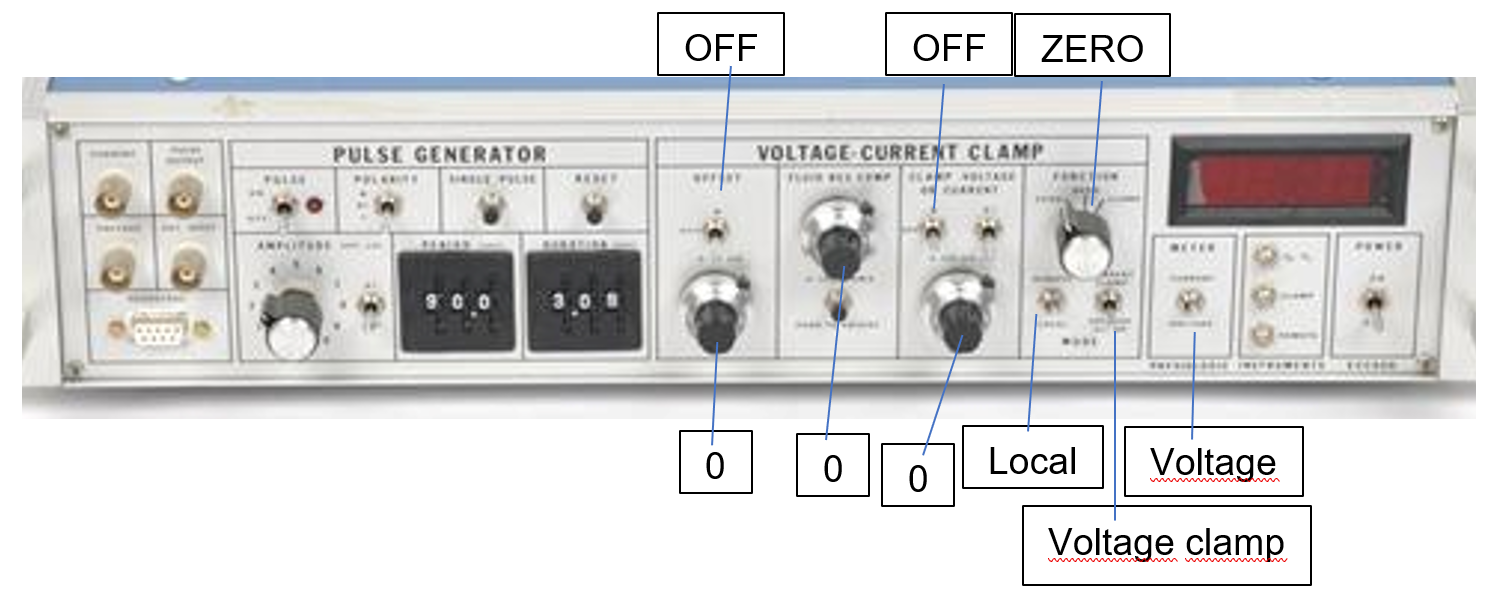
\includegraphics[width=20.86in]{images/Equipment settings}

\section{Get familiar with the two measuring modes}\label{get-familiar-with-the-two-measuring-modes}

Your equipment has to be on the rest setting at all times, unless you want to measure something. We will continuously measure voltage and current. For that you have to switch between two instrument settings. Familiarize yourself with both procedures.

\subsection{Measure Voltage}\label{measure-voltage}

\begin{enumerate}
\def\labelenumi{\arabic{enumi}.}
\item
  Set the FUNCTION switch to OPEN and METER to VOLTAGE
\item
  Read the value in the display
\end{enumerate}

\subsection{Measure Current}\label{measure-current}

\begin{enumerate}
\def\labelenumi{\arabic{enumi}.}
\item
  Set the FUNCTION switch to CLAMP and METER to CURRENT
\item
  Read the value in the display
\end{enumerate}

\section{Account for electrode asymmetry}\label{account-for-electrode-asymmetry}

\begin{enumerate}
\def\labelenumi{\arabic{enumi}.}
\item
  Switch FUNCTION to OPEN, and METER to VOLTAGE. The value that is now displayed reflects the asymmetry of the electrodes.
\item
  Use the OFFSET SWITCH in the plus or minus position and turn the OFFSET DIAL to bring the number on the display to zero.
\item
  If it doesn't work, get help. Check for air bubbles in your voltage electrodes (black).
\end{enumerate}

\section{Account for fluid resistance}\label{account-for-fluid-resistance}

\begin{enumerate}
\def\labelenumi{\arabic{enumi}.}
\item
  Function switch still on OPEN, place METER to CURRENT and hold the FLUID RESISTANCE COMPENSATION button down.
\item
  The values should now be between 60 and 68 µA.
\item
  If it is lower, your resistance is too high. Get help.
\item
  Still holding the button switch to voltage mode (OPEN + VOLTAGE). Adjust the fluid resistance compensation dial to bring the number on the display to zero.
\item
  The value on the dial represents the fluid resistance of your system. I.e. the resistance all fluid parts of the setup together have.
\item
  Note down the fluid resistance.
\end{enumerate}

\section{Mount skin sample}\label{mount-skin-sample}

\textbf{OBS: After mounting the skin sample, you have to immediately start measuring I and V, so get ready for that first}

\begin{enumerate}
\def\labelenumi{\arabic{enumi}.}
\item
  Empty your chamber using the provided syringe.
\item
  Get a skin sample that was dissected from green frogs ( \emph{Rana kl. esculentus} ). The skin was dissected from different parts of the frog (e.g.~belly, back, leg etc). Note down from which part your skin was.
\item
  Identify the outer (mucosal) and inner (serosal) side.
\item
  Mount the skin on the slider of the Ussing chamber. Try to have the mucosal side point to the left halfchamber. It is important to keep track which side points to which half-cell of the chamber!
\item
  Note down to which side the mucosal side points.
\item
  Fill fresh Ringer's solution into both half chambers and ensure that both sides are bubbled. The stream of air bubble serves two purposes: it provides oxygen and mixing of the Ringer's solution.
\item
  Check for leaks.
\item
  Check for air bubbles in the chamber and specifically on the skin.
\item
  Start your stopwatch.
\end{enumerate}

\chapter{Experiment 1: Determine the epithelial resistance}\label{experiment-1-determine-the-epithelial-resistance}

You will now measure the potential difference over the skin (from now on referred to as V) as well as the current needed to even out the potential difference between both sides (from now on referred to as I). This current is also called ''short circuit current''. I is a measure of ion transport across the skin.

\section{Take measurements}\label{take-measurements}

Measure V and I every minute for 10 minutes after mounting the skin.

\begin{enumerate}
\def\labelenumi{\arabic{enumi}.}
\item
  Measure V and note it in your excel sheet.
\item
  Measure I and note it in your excel sheet.
\item
  Repeat for 10 minutes in 1 minute intervals.
\end{enumerate}

\textbf{When not taking measurements, always switch to ZERO.}

\section{Data analysis}\label{data-analysis}

The value we would like to measure is the resistance of the skin, so we need to calculate the measurements you made.

Use Ohm's law to calculate the electrical resistance R of the skin. Make sure to get the unit right.

\section{Discussion}\label{discussion}

Once you have calculated the reistance, try to answer the questions below. We will discuss them in the group, and you will use them to guide your data discussion for the report.

\begin{enumerate}
\def\labelenumi{\arabic{enumi}.}
\item
  What does the epithelial resistance reflect?
\item
  What is the unit of the resistance?
\item
  How can we make it more comparable across experiments?
\end{enumerate}

\begin{itemize}
\tightlist
\item
  How are these parameters called?
\end{itemize}

\begin{enumerate}
\def\labelenumi{\arabic{enumi}.}
\setcounter{enumi}{3}
\item
  Do the values change over time?
\item
  What can we conclude from that?
\item
  What is the mechanism behind our observations? Why?
\end{enumerate}

\chapter{Experiment 2: Concentration dependence of ion transport}\label{experiment-2-concentration-dependence-of-ion-transport}

In this experiment, you will investigate whether the ion transport process depends on the concentration of sodium ions on the mucosal side. To achieve this, you will measure I for a series of diluted Ringer's solutions. The 1x Ringers you used so far was \textbf{112 mM NaCl}.

\section{Preparation}\label{preparation}

What is the concentration of Na\textsuperscript{+}-ions in 1x Ringer's?

To test if the ion transport depends on the concentration of Na\textsuperscript{+}-ions, we will need the following solutions:

Calculate the different concentrations of Na\textsuperscript{+}-ions yourself and enter them in the \textbf{excel sheet}.
Plan how to prepare 20 mL of each of these solutions from 1x or 2x Ringer's. Once you have a plan find an instructor to help you make the solutions.

\section{Take measurements}\label{take-measurements-1}

\begin{enumerate}
\def\labelenumi{\arabic{enumi}.}
\item
  Empty chamber
\item
  Using the 0x solution, wash the chamber on the mucosal side 3 times (wait 2 minutes in-between).
\item
  Measure I and note it in your excel sheet.
\item
  Empty the chamber and add the solution with the next higher concentration.
\item
  Wait 1 minute
\item
  Measure I and note it in your excel sheet.
\item
  Repeat step 4-6 for each of the solutions in order of increasing Na\textsuperscript{+}-ion concentration.
\item
  \textbf{At the end go back to 1x Ringer's!}
\end{enumerate}

\section{Data Analysis}\label{data-analysis-1}

\begin{enumerate}
\def\labelenumi{\arabic{enumi}.}
\item
  Convert I to the flux of Na+-ions (J) using the following relationship (F: Farraday constant):
  \(J_{Na^+} = \frac {I_{Na^+}}{F} = \frac {1\frac {C} {s}} {96500 \frac {C} {mol}}\)
\item
  Plot J as a function of Na\textsuperscript{+}-concentration.
\end{enumerate}

\section{Discussion}\label{discussion-1}

\begin{enumerate}
\def\labelenumi{\arabic{enumi}.}
\item
  Have you seen a curve like that before? What is it called?
\item
  What kind of information can you extract from these curves?
\end{enumerate}

\chapter{Experiment 3: Influence of chloride ions}\label{experiment-3-influence-of-chloride-ions}

In this experiment, you investigate whether overall ion exchange over the membrane includes chloride ions. To characterize the anion transport, you will use ``Sulfate - Ringer's solution'' on the mucosal side of the skin. In ``Sulfate - Ringer's'', chloride ions are replaced with SO\textsubscript{4}\textsuperscript{2}- ions.

To compare normal ringers to Sulfate-Ringers, we will take the average of 5 measurements

\section{Take measurements}\label{take-measurements-2}

\begin{enumerate}
\def\labelenumi{\arabic{enumi}.}
\item
  Empty chamber on mucosal side.
\item
  Using 1x Ringer's, wash the chamber on the mucosal side 3 times (wait 2 minutes in-between).
\item
  Measure V and note it in your excel sheet.
\item
  Measure I and note it in your excel sheet.
\item
  Repeat (step 3-4 for) 4 times in 1 minute intervals.
\item
  Empty chamber on mucosal side.
\item
  Using Sulfate Ringer's, wash the chamber on the mucosal side 3 times (wait 2 minutes in-between).
\item
  Measure V and note it in your excel sheet.
\item
  Measure I and note it in your excel sheet.
\item
  Repeat (step 8-9 for) 4 times in 1 minute intervals.
\end{enumerate}

\section{Discussion}\label{discussion-2}

\begin{enumerate}
\def\labelenumi{\arabic{enumi}.}
\tightlist
\item
  What happened after changing the buffer?
\item
  Why?
\item
  What are the underlying mechanisms?
\end{enumerate}

\chapter{Instructions for your lab report}\label{instructions-for-your-lab-report}

\textbf{Introduction:} Describe how a frog osmoregulates in its natural habitat. Pay special attention to describing how the cells mechanistically function. Name and highlight the most important ion transporters the frog is using to stay in homeostasis. Remember to include a brief objective at the end. Max. 1 page.

\textbf{Methods:} with drawing/pictures/figures of the arrangement. Provide a general ovewrview of the experiment and pay attention to describe and mention any deviations from the manual. The figures can be made in the program BioRender (www.biorender.com).

\textbf{Results:} relevant figures/tables (from all experiments) with accompanying explanation; the main trends/effects in the figures are described in words. It is good practice to end the paragraph related to a figure with the main take home message of the figure. Remember that you do not discuss/explain anything in the results section, you only must describe.

\textbf{Discussion:} of results and conclusion (see guidance questions below). What have you shown? How does this fit in with the theoretical background? Assess and discuss uncertainties and sources of error.

\textbf{Conclusion}

Include your R-script as *.R file and your excel sheets in the upload.

Hand in as group and remember to include all members' full names and email addresses.

The hand-in date for the report is indicated in the assignment on ItsLearning.

\textbf{General form}
For this lab report I expect you to adhere to all good practice regarding figures, quantitative reporting, scientific language, writing and practice that you have learned since you started studying Biology. As a guide you can refer to the guidelines for report writing you have been using many times before (linked in the assignment).

\section{Questions and points that should be adressed in the report}\label{questions-and-points-that-should-be-adressed-in-the-report}

Experiment 1:

\begin{enumerate}
\def\labelenumi{\arabic{enumi}.}
\item
  What does the epithelial resistance reflect?
\item
  What is the unit of the resistance? (Make sure to have that right in the report)
\item
  How can we make it more comparable across experiments?
\end{enumerate}

\begin{itemize}
\tightlist
\item
  How are these parameters called? (Make sure to use these throughout the entire report)
\end{itemize}

\begin{enumerate}
\def\labelenumi{\arabic{enumi}.}
\setcounter{enumi}{3}
\item
  Do the values change over time?
\item
  What can we conclude from that?
\item
  What is the mechanism behind our general observations? Why?
\end{enumerate}

Experiment 2:

\begin{enumerate}
\def\labelenumi{\arabic{enumi}.}
\item
  Have you seen a curve (Na-flux over Na-concentration) like that before? What is it called?
\item
  What kind of information can you extract from these curves?
\item
  What does K\textsubscript{m} express?
\item
  What does V\textsubscript{max} express?
\item
  Based on your results: Give an estimate of how fast the transport (in \% of V\textsubscript{max}) takes place when a frog is sitting in its watering hole, with a Na\textsuperscript{+}-concentration of approximately 5 mmol/L.
\end{enumerate}

Experiment 3:

\begin{enumerate}
\def\labelenumi{\arabic{enumi}.}
\item
  What happened after changing the buffer?
\item
  Why?
\item
  What are the underlying mechanisms?
\end{enumerate}

\chapter{Analyzing your data}\label{analyzing-your-data}

In order to strengthen your programming and data analysis skills, we will analyze the data for this course in R. If you are proficient enough in another programming language or environment and can produce the same outcome there, that is fine with me too.

This chapter will take you through all the steps analyzing and visualizing your data and link to little instructions how do do this in R. You do not get a prewritten script, but should write your own with the instructions provided here as well as your knowledge from previous courses (eg statistics).

\section{Experiment 1:}\label{experiment-1}

The value we would like to measure in this exercise is the resistance of the skin, so we need to calculate it from the measurements you made.

\begin{enumerate}
\def\labelenumi{\arabic{enumi}.}
\item
  Read your data into R. See \ref{reading}
\item
  Use Ohm's law to calculate the electrical resistance R of the skin. Make sure to get the unit right. For example:
\end{enumerate}

\begin{Shaded}
\begin{Highlighting}[]
\NormalTok{data1}\SpecialCharTok{$}\NormalTok{R }\OtherTok{\textless{}{-}}\NormalTok{ (data1}\SpecialCharTok{$}\NormalTok{V}\SpecialCharTok{*}\DecValTok{1000}\NormalTok{)}\SpecialCharTok{/}\NormalTok{data1}\SpecialCharTok{$}\NormalTok{I}
\end{Highlighting}
\end{Shaded}

\begin{enumerate}
\def\labelenumi{\arabic{enumi}.}
\setcounter{enumi}{2}
\tightlist
\item
  Calculate resistivity and current density.
\end{enumerate}

\begin{Shaded}
\begin{Highlighting}[]
\NormalTok{data}\SpecialCharTok{$}\NormalTok{R\_cm2 }\OtherTok{\textless{}{-}}\NormalTok{ data}\SpecialCharTok{$}\NormalTok{R }\SpecialCharTok{/} \FloatTok{0.71}
\NormalTok{data}\SpecialCharTok{$}\NormalTok{I\_cm2 }\OtherTok{\textless{}{-}}\NormalTok{ data}\SpecialCharTok{$}\NormalTok{I }\SpecialCharTok{/} \FloatTok{0.71}
\end{Highlighting}
\end{Shaded}

\begin{enumerate}
\def\labelenumi{\arabic{enumi}.}
\setcounter{enumi}{3}
\tightlist
\item
  Plot resistivity and current density over time see \ref{plotting}
\end{enumerate}

\section{Experiment 2:}\label{experiment-2}

\begin{enumerate}
\def\labelenumi{\arabic{enumi}.}
\item
  Read your data into R. See \ref{reading}
\item
  Convert I to the flux of Na+-ions (J) using the following relationship (F: Farraday constant):
  \(J_{Na^+} = \frac {I_{Na^+}}{F} = \frac {1\frac {C} {s}} {96500 \frac {C} {mol}}\)
\item
  Plot J as a function of Na\textsuperscript{+}-concentration. \ref{plotting}
\end{enumerate}

\subsection{\texorpdfstring{Extract V\textsubscript{max} and K\textsubscript{m} using nonlinear curve fitting.}{Extract Vmax and Km using nonlinear curve fitting.}}\label{extract-vmax-and-km-using-nonlinear-curve-fitting.}

One of the advantages of having modern computers is that we can do curve fitting to non-linear functions. We will apply this to find the V\textsubscript{max} and K\textsubscript{m} of your data.

\begin{enumerate}
\def\labelenumi{\arabic{enumi}.}
\tightlist
\item
  First we have to define the equation we want to use. We are using the Michaelis Menten formula:
\end{enumerate}

\(V_0 = \frac {V_{max} * S}{K_m + S}\)

\begin{Shaded}
\begin{Highlighting}[]
\NormalTok{MMcurve }\OtherTok{\textless{}{-}} \FunctionTok{formula}\NormalTok{(J }\SpecialCharTok{\textasciitilde{}}\NormalTok{ Vmax }\SpecialCharTok{*}\NormalTok{ Na\_concentration }\SpecialCharTok{/}\NormalTok{ (Km }\SpecialCharTok{+}\NormalTok{ Na\_concentration))}
\end{Highlighting}
\end{Shaded}

\begin{enumerate}
\def\labelenumi{\arabic{enumi}.}
\setcounter{enumi}{1}
\tightlist
\item
  Next we will use the R curve fitting function nls() to find the V\textsubscript{max} and K\textsubscript{m} that will best fit our measured values to the Michaelis-Menten-equation. For that we have to provide some start values for the function to use.
\end{enumerate}

\begin{Shaded}
\begin{Highlighting}[]
\NormalTok{bestfit }\OtherTok{\textless{}{-}} \FunctionTok{nls}\NormalTok{(MMcurve, data2, }\AttributeTok{start =} \FunctionTok{list}\NormalTok{(}\AttributeTok{Vmax =} \DecValTok{50}\NormalTok{, }\AttributeTok{Km =} \DecValTok{2}\NormalTok{))}
\end{Highlighting}
\end{Shaded}

\begin{enumerate}
\def\labelenumi{\arabic{enumi}.}
\setcounter{enumi}{2}
\tightlist
\item
  Now we will calculate the fitted curve for Na\textsuperscript{+}-ion concentrations from 0 mM to 170 mM.
\end{enumerate}

\begin{Shaded}
\begin{Highlighting}[]
\CommentTok{\#create many x{-}values from 0 to 170}
\NormalTok{Na\_conc }\OtherTok{\textless{}{-}} \FunctionTok{seq}\NormalTok{(}\DecValTok{0}\NormalTok{,}\DecValTok{170}\NormalTok{,}\FloatTok{0.1}\NormalTok{) }
\CommentTok{\#calculate the y{-}values using the fitted function}
\NormalTok{J\_fitted }\OtherTok{\textless{}{-}} \FunctionTok{predict}\NormalTok{(bestfit,}\FunctionTok{list}\NormalTok{(}\AttributeTok{Na\_concentration =}\NormalTok{ Na\_conc))}
\end{Highlighting}
\end{Shaded}

\begin{enumerate}
\def\labelenumi{\arabic{enumi}.}
\setcounter{enumi}{3}
\tightlist
\item
  Now we plot our real data and add the fitted values
\end{enumerate}

\begin{Shaded}
\begin{Highlighting}[]
\FunctionTok{plot}\NormalTok{(FILL THIS OUT YOURSELF)}
\NormalTok{test }\OtherTok{\textless{}{-}} \FunctionTok{lines}\NormalTok{(Na\_conc, J\_fitted)}
\end{Highlighting}
\end{Shaded}

\begin{enumerate}
\def\labelenumi{\arabic{enumi}.}
\setcounter{enumi}{4}
\tightlist
\item
  Now we only need to extract the values for V\textsubscript{max} and K\textsubscript{m} from the fitted equation. The values are stored in ``bestfit'' and you can extract them like this:
\end{enumerate}

\begin{Shaded}
\begin{Highlighting}[]
\NormalTok{Vmax }\OtherTok{\textless{}{-}} \FunctionTok{coef}\NormalTok{(bestfit)[}\DecValTok{1}\NormalTok{]}
\NormalTok{Km }\OtherTok{\textless{}{-}} \FunctionTok{coef}\NormalTok{(bestfit)[}\DecValTok{2}\NormalTok{]}
\NormalTok{Vmax}
\NormalTok{Km}
\end{Highlighting}
\end{Shaded}

\section{Experiment 3}\label{experiment-3}

\begin{enumerate}
\def\labelenumi{\arabic{enumi}.}
\item
  Read in your data. See \ref{reading}
\item
  Calculate resistivity, current density and resistance for both conditions.
\item
  Take the average of all values from one condition. See \ref{averaging}
\item
  Plot potential difference, current density and resistivity of the two groups. See \ref{plotting}
\end{enumerate}

\chapter{R instructions and help to solve p-R-oblems}\label{r-instructions-and-help-to-solve-p-r-oblems}

\section{How to\ldots{}}\label{how-to}

\subsection{Read in data}\label{reading}

Depending on how your computer is set up, csv files require different settings to read in.
A CSV file is simply a text file, where columns are separated by one sign and the decimal point is indicated by another. In English speaking countries and most scientific data you can download from the internet, columns are separated by a comma ``,'' and the decimal point is a ``.''. The default in other European countries, including Denmark, is to use a semikolon ``;'' to separate columns and a comma ``,'' as decimal point.

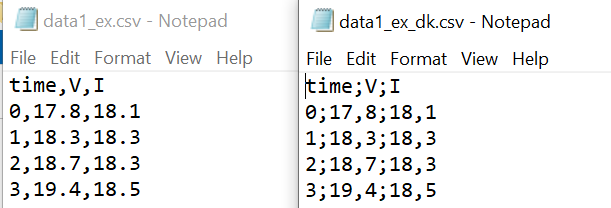
\includegraphics[width=8.49in]{images/CSV comparison}

Depending on which settings your computer follows, you will have to read in csv files using two different functions:

Reading in data from ``Danish files'':

\begin{Shaded}
\begin{Highlighting}[]
\NormalTok{data }\OtherTok{\textless{}{-}} \FunctionTok{read.csv2}\NormalTok{(}\StringTok{"folder/myfile.csv"}\NormalTok{)}
\end{Highlighting}
\end{Shaded}

Reading in data from ``English files'':

\begin{Shaded}
\begin{Highlighting}[]
\NormalTok{data }\OtherTok{\textless{}{-}} \FunctionTok{read.csv}\NormalTok{(}\StringTok{"folder/myfile.csv"}\NormalTok{)}
\end{Highlighting}
\end{Shaded}

Many errors are related to this step.
See \ref{e1}

\subsection{Plot your data}\label{plotting}

The basic plot command in R is plot().
You HAVE to tell the function:
- what to put on the x-axis,
- and the y-axis,
And you CAN tell the function additionally:
- which type of plot you want,
- what the axis labels should be and
- the min and max points of the axes.

\begin{Shaded}
\begin{Highlighting}[]
\FunctionTok{plot}\NormalTok{(}\AttributeTok{x =}\NormalTok{ data1}\SpecialCharTok{$}\NormalTok{time, }
     \AttributeTok{y =}\NormalTok{ data1}\SpecialCharTok{$}\NormalTok{V, }
     
     \AttributeTok{type =} \StringTok{"l"}\NormalTok{,}
     \AttributeTok{xlab =} \StringTok{"Time (min)"}\NormalTok{, }
     \AttributeTok{ylab =} \StringTok{"Potential difference (mV)"}\NormalTok{,}
     \AttributeTok{ylim =} \FunctionTok{c}\NormalTok{(}\DecValTok{0}\NormalTok{, }\FunctionTok{max}\NormalTok{(data1}\SpecialCharTok{$}\NormalTok{V)))}
\end{Highlighting}
\end{Shaded}

\subsection{Averaging by group}\label{averaging}

Often you want to calculate the average and standard deviation of a dataset by group. Below is one way of doing this for all data in one command using the aggregate function. You tell it how the average should be named (av\_V), what it should be calculated from (data\$V), and if there is a column that informs about the grouping (by = data\$condition) and which function you want to apply(FUN = mean).

\begin{Shaded}
\begin{Highlighting}[]
\CommentTok{\#calculating all averages}
\NormalTok{data\_av }\OtherTok{\textless{}{-}} \FunctionTok{aggregate}\NormalTok{(}\FunctionTok{list}\NormalTok{(}\AttributeTok{av\_V =}\NormalTok{ data}\SpecialCharTok{$}\NormalTok{V, }
                          \AttributeTok{av\_R\_cm2 =}\NormalTok{ data}\SpecialCharTok{$}\NormalTok{R\_cm2, }
                          \AttributeTok{av\_I\_cm2 =}\NormalTok{ data}\SpecialCharTok{$}\NormalTok{I\_cm2),}
                     \FunctionTok{list}\NormalTok{(data}\SpecialCharTok{$}\NormalTok{condition), }
                     \AttributeTok{FUN =}\NormalTok{ mean )}

\CommentTok{\#calculating all standard deviations}
\NormalTok{data\_sd }\OtherTok{\textless{}{-}} \FunctionTok{aggregate}\NormalTok{(}\FunctionTok{list}\NormalTok{(}\AttributeTok{sd\_V =}\NormalTok{ data}\SpecialCharTok{$}\NormalTok{V, }
                          \AttributeTok{sd\_R\_cm2 =}\NormalTok{ data}\SpecialCharTok{$}\NormalTok{R\_cm2, }
                          \AttributeTok{sd\_I\_cm2 =}\NormalTok{ data}\SpecialCharTok{$}\NormalTok{I\_cm2),}
                     \FunctionTok{list}\NormalTok{(data3}\SpecialCharTok{$}\NormalTok{condition), }
                     \AttributeTok{FUN =}\NormalTok{ sd )}

\CommentTok{\#then we attach the sd columns to the table that has the means}
\NormalTok{data\_mean }\OtherTok{\textless{}{-}} \FunctionTok{cbind}\NormalTok{(data3\_av, data3\_sd[}\DecValTok{2}\SpecialCharTok{:}\DecValTok{4}\NormalTok{])}
\end{Highlighting}
\end{Shaded}

\subsection{Set your working directory to a different folder}\label{setwd}

The working directory is the place ``where R works from'' at the moment. Files that are in that folder can be used by simply using their file name. If you need to change to a different folder, there are two ways:
1. commandline

\begin{Shaded}
\begin{Highlighting}[]
\FunctionTok{setwd}\NormalTok{(}\StringTok{"C:/Users/new/path/to/folder/you/want"}\NormalTok{)}
\end{Highlighting}
\end{Shaded}

\begin{enumerate}
\def\labelenumi{\arabic{enumi}.}
\setcounter{enumi}{1}
\tightlist
\item
  Using R studio interface
\end{enumerate}

\begin{enumerate}
\def\labelenumi{\alph{enumi})}
\tightlist
\item
  Go to ``Files''
\item
  Navigate to the folder you want to use as new working directory
\item
  Click on the settings wheel
\item
  Click ``Select As Working Directory''
\item
  Done :)
\end{enumerate}

\subsection{Write and troubleshoot a new script}\label{write-and-troubleshoot-a-new-script}

\begin{enumerate}
\def\labelenumi{\arabic{enumi}.}
\tightlist
\item
  Think about what you want the code to do.
\item
  Identify the functions that you need.
\item
  Start writing your code.
\item
  Check if the code did what you expected after every step.
  The last step is really important. You can run scripts without ever seeing your data and R will do whatever you tell it, no matter whether it makes sense or not. When writing new code, it is vital to check the result after each step.
\end{enumerate}

Usefull check are:
Simply view the data table or object you work on to see the result of your code

\begin{Shaded}
\begin{Highlighting}[]
\FunctionTok{View}\NormalTok{(df)}
\end{Highlighting}
\end{Shaded}

Check if the table or column has the right type of data in it.

str() tells you what kind of table df is, how many rows (the number of objects) and columns (the number of variables) there are, and what type of data is in the columns. It is a very useful tool for troubleshooting:
- Does your data frame have the right amount of columns? Lets say you calculated a new variable and wrote it into a column, then there should be one more than before
- Does your data frame have the right amount of rows?
- Is the data in the right format? ``chr'' means that the column is a character column, which means it is regarded as text. Even if the signs are numbers, R will not be able to use the column for calculations.

\begin{Shaded}
\begin{Highlighting}[]
\FunctionTok{str}\NormalTok{(df)}
\end{Highlighting}
\end{Shaded}

\subsection{Change the type of data in a column}\label{change-the-type-of-data-in-a-column}

Most commonly you want to do this if R has read in data as ``character'' (text), but you need it to be ``numeric'' (numbers).
Of note: Typically, if you have a column that should be numeric but isn't, then there is a problem when reading in the data or creating the column taht should be solved.

Changing a column from ``character'' to ``numeric'':

\begin{Shaded}
\begin{Highlighting}[]
\NormalTok{df}\SpecialCharTok{$}\NormalTok{col }\OtherTok{\textless{}{-}} \FunctionTok{as.numeric}\NormalTok{(data}\SpecialCharTok{$}\NormalTok{col)}
\CommentTok{\#Takes the column "col" in the table df, formats it as number and overwrites it with itself. }
\end{Highlighting}
\end{Shaded}

\section{Common error messages and how to solve them}\label{common-error-messages-and-how-to-solve-them}

\subsection{Cannot open the connection}\label{e1}

\subsubsection*{The error}\label{the-error}
\addcontentsline{toc}{subsubsection}{The error}

When you try to read in a csv file you get the error message below:

\begin{Shaded}
\begin{Highlighting}[]
\FunctionTok{read.csv}\NormalTok{(}\StringTok{"data2.csv"}\NormalTok{)}
\end{Highlighting}
\end{Shaded}

\begin{verbatim}
## Warning in file(file, "rt"): cannot open file 'data2.csv': No such file or directory
\end{verbatim}

\begin{verbatim}
## Error in file(file, "rt"): cannot open the connection
\end{verbatim}

\subsubsection*{Why is this happening?}\label{why-is-this-happening}
\addcontentsline{toc}{subsubsection}{Why is this happening?}

You just told R to open a file in your working directory that is called data2.csv. R is telling you it can't do that because the file doesn't exist. The two major reasons for this are:
1. The file is in a different folder.
2. You mistyped the filename.

\subsubsection*{Troubleshooting}\label{troubleshooting}
\addcontentsline{toc}{subsubsection}{Troubleshooting}

\begin{enumerate}
\def\labelenumi{\arabic{enumi}.}
\tightlist
\item
  Check where your current working directory is set to.
\end{enumerate}

\begin{Shaded}
\begin{Highlighting}[]
\FunctionTok{getwd}\NormalTok{()}
\end{Highlighting}
\end{Shaded}

Is the file in the working directory?

Yes: check for correct spelling.

No: Either use the path to the file in the command OR change the working directory to the folder where the file is in as described in \ref{setwd}.

\subsection{My code doesn't do what it should or fails with cryptic message}\label{my-code-doesnt-do-what-it-should-or-fails-with-cryptic-message}

\begin{enumerate}
\def\labelenumi{\arabic{enumi}.}
\tightlist
\item
  Google
\item
  If you are taking BB511 at the moment: Ask Iris :)
\end{enumerate}

  \bibliography{book.bib,packages.bib}

\end{document}
